The transform between joint adjacent joints is represented by the transform:

\begin{equation}\label{eq:dhT}
T_{i-1}^{i} = \left[ \begin{array}{cccc} 
cos(\theta_i) & -sin(\theta_i)cos(\alpha_i) &  sin(\theta_i)sin(\alpha_i)  &  a_i cos(\theta_i) \\ 
sin(\theta_i) &  cos(\theta_i)cos(\alpha_i) & -cos(\theta_i)sin(\alpha_i)  &  a_i sin(\theta_i) \\
0             &  sin(\alpha_i)              &  cos(\alpha_i)               &  d_i               \\
0             &  0                          &  0                           &  1                 
\end{array} \right]
\end{equation}

Where $\theta_i$, $\alpha_i$ and $d_i$ are shown in Fig.~\ref{fig:dhDiagram}.  The coordinate frame of the Hubo2+ used for both the forward and inverse kinematics are defined in Fig.~\ref{fig:IkFkCoordinate}.  The DH parameters for the arm for the transform $T_i^{i-1}$ is found in Table~\ref{table:dhparamrightArm}.

\begin{figure}[thpb]
  \centering
%  \begin{minipage}{\textwidth}
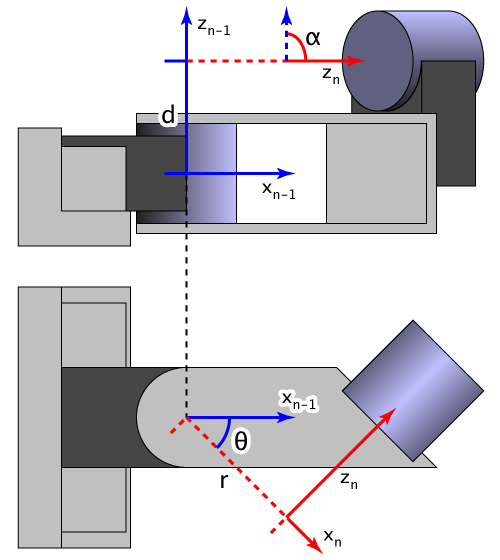
\includegraphics[width=0.5\columnwidth]{./examples/pix/Sample_Denavit-Hartenberg_Diagram.png}
\caption{Denavit-Hartenberg diagram showing that axis of rotations and displacements to create the transform in Equation~\ref{eq:dhT}.  $\alpha$ is the angle between the axis of rotation of joint $n$ and $n-1$ about the of $n$. $\theta$ is the angle between the axis of rotation of joint $n$ and $n-1$ about the axis perpendicular to the axis about $n$.}
Image Credit: \textit{http://en.wikipedia.org/wiki/File:Sample\_Denavit-Hartenberg\_Diagram.png}
\label{fig:dhDiagram}
%  \end{minipage}
\end{figure}


\begin{figure}[thpb]
  \centering
%  \begin{minipage}{\textwidth}
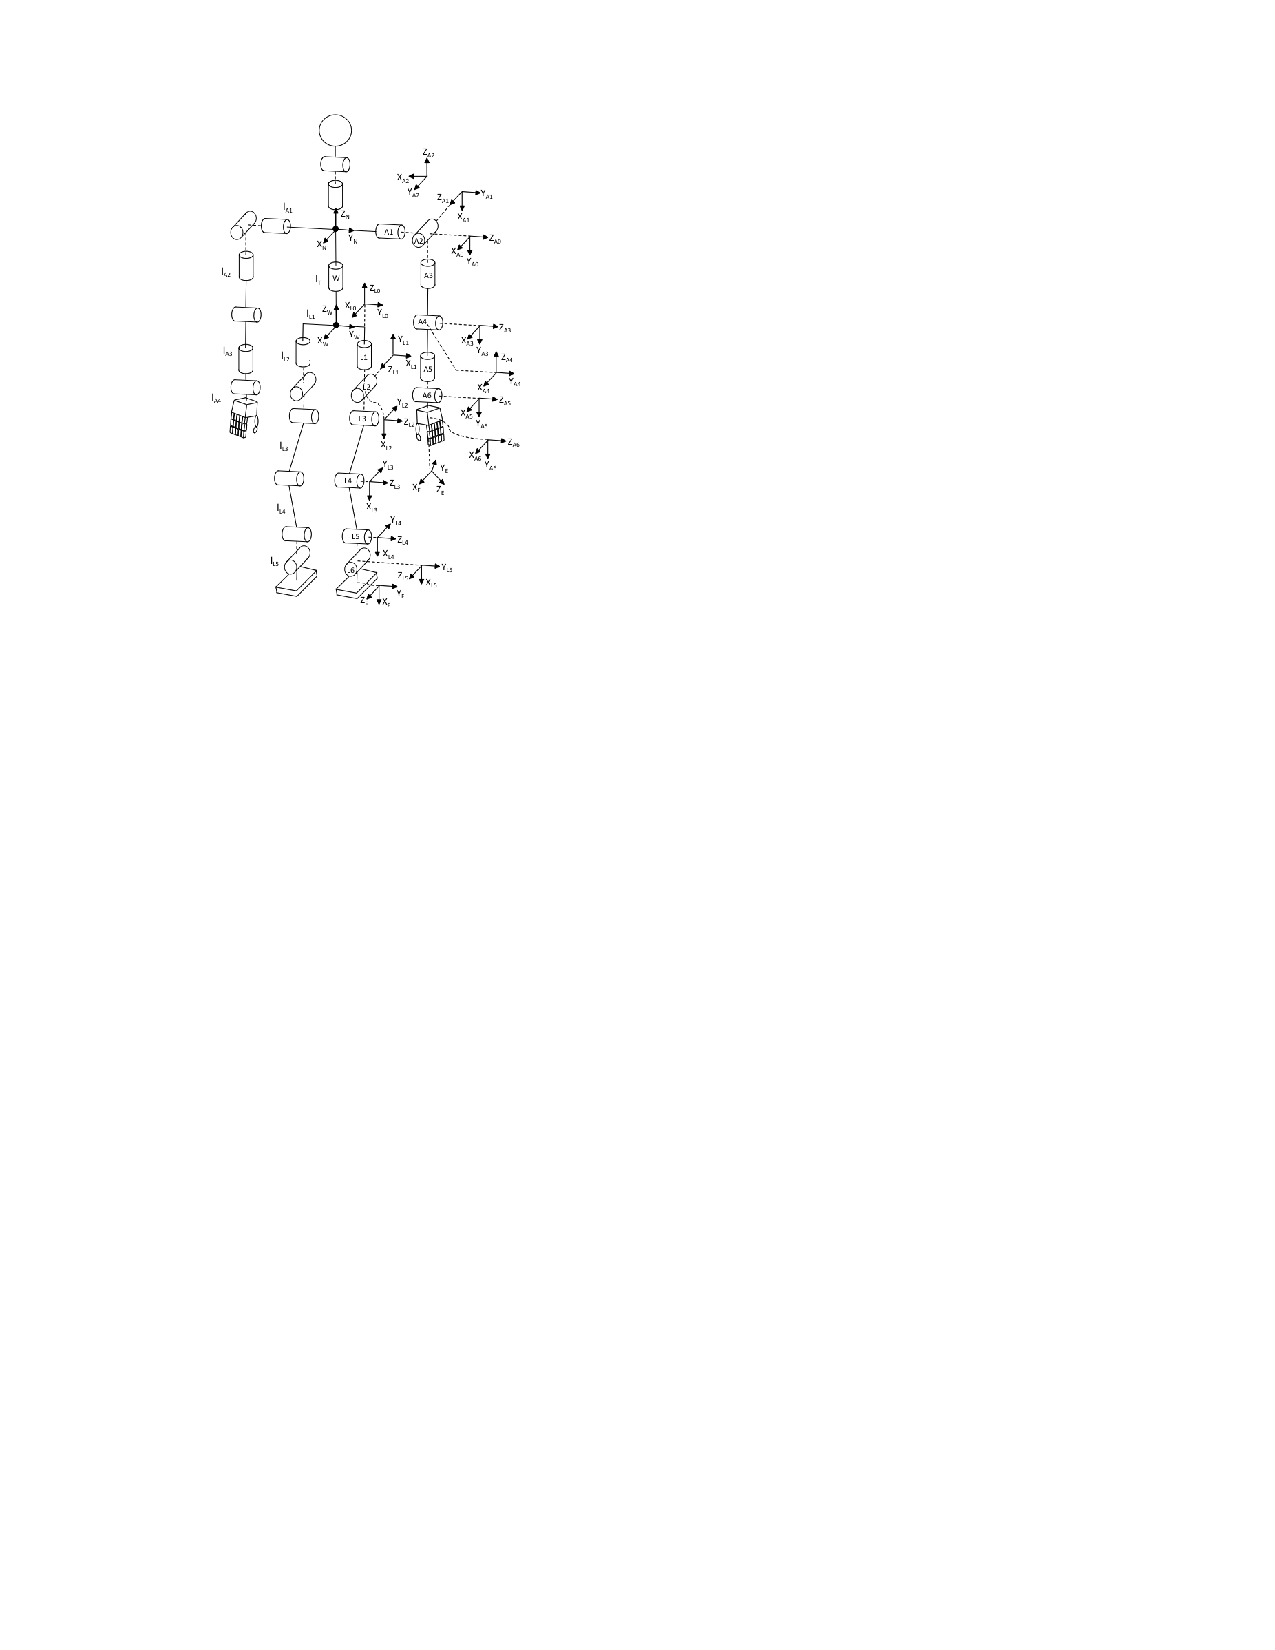
\includegraphics[width=0.8\columnwidth]{./examples/pix/hubo2GTechFrame.pdf}
\caption{Hubo2+ coordinate frame for use with the forward and inverse kinematic example.  These coordinate frames are defigned spisificall for IK and FK     }
\label{fig:IkFkCoordinate}
%  \end{minipage}
\end{figure}


\begin{table}
\centering
\caption{Denavit–Hartenberg Parameters (continued) for Hubo2+ upper body (arms) in standard format}
\begin{tabular}{| c || c | c | c | c|}
\hline
$i$ (frame)  & $\theta_i$ (rad)         & $\alpha_i$ (rad) & $a_i$ (m) & $d_i$ (m) \\
\hline
\hline
1            & $\theta_1+\frac{\pi}{2}$ & $\frac{\pi}{2}$  & 0         & 0          \\
\hline
2            & $\theta_2-\frac{\pi}{2}$ & $\frac{\pi}{2}$  & 0         & 0          \\
\hline
3            & $\theta_3+\frac{\pi}{2}$ & $-\frac{\pi}{2}$ & 0         & $-l_{A2}$  \\
\hline
4            & $\theta_4$               & $\frac{\pi}{2}$  & 0         & 0          \\
\hline
5            & $\theta_5$               & $\frac{\pi}{2}$  & 0         & $-l_{A3}$  \\
\hline
6            & $\theta_6+\frac{\pi}{2}$ & 0                & $l_{A4}$  & 0          \\

\hline

\end{tabular}\label{table:dhparamrightArm}
\end{table}

In order to calculate for full FK transform $T_{N}^{E}$, where $E$ represents the end-effector and $N$ is the neck (robot origin), we must first calculate:

\begin{equation}\label{eq:t06}
T_0^6 = \prod_{i=1}^{5} T_{i-1}^{i} T_{i}^{i+1} = T_{0}^{1}T_{1}^{2}T_{2}^{3}T_{3}^{4}T_{4}^{5}T_{5}^{6}
\end{equation}

In order to procure the transform $T_{N}^{E}$ we must pre-multiply $T_{0}^{6}$ by the transform $T_{N}^{0}$ and post-multiply it by the transform $T_{6}^{E}$.  
This results in transform $T_{N}^{E}$:

\begin{equation}
T_{N}^{E} = T_{N}^{0}T_{0}^{6}T_{6}^{E}
\end{equation}

Where $T_{N}^{0}$ is

\begin{equation}
T_{N}^{0} = \left[ \begin{array}{cccc} 
0 & 0 & 1 &  l_{A1} \\ 
1 & 0 & 0 &  0        \\
0 & 1 & 0 &  0        \\
0 & 0 & 0 &  1                 
\end{array} \right]
\end{equation} 


Now with a given set of joint space angles we can find the end-effectors position in reference to the robot origin, the neck.
